\documentclass[UTF8]{ctexart}

\usepackage{WeeklyReport}
\usepackage{graphicx}
\usepackage{amsmath}
\usepackage{amssymb}

\title{周报03}
\author{傅阳烨}
\date{\today}

\begin{document}
    \maketitle
    % \tableofcontents
    \section{学习内容}
        \begin{itemize}
            \item 整理思路,设计Loss
        \end{itemize}
    \section{学习收获}
        这次主要的做的事情是把之前的一些零散的想法整理一下,尝试进行Loss的设计
        \subsection{部分匹配损失Partial Alignment Loss}
            某一个source可能并不包含target的所有feature,而某些feature是包含的。
            不同source组合起来则可以包含target的所有feature,
            因此考虑target对不同source的不同(部分)feature进行alignment。
            在feature space中,可能的情况如图 \ref{fig:feature} 所示,
            因此target在与source匹配时,只需要匹配一部分的feature。
            \begin{figure}[ht]
                \centering
                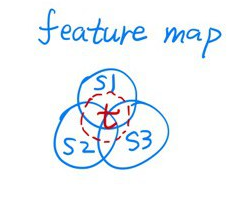
\includegraphics{Week03_feature.png}
                \caption{在feature space中可能的情况}
                \label{fig:feature}
            \end{figure}
            \subsubsection{公式推导}
                传统的做法是对所有source进行alignment,即normalize之后,
                直接与target计算差异,在partial alignment的情况下,
                只需要计算某些维度上的loss。以下讨论针对batch size为1的情况:

                假设特征提取后得到的是一个 $n$ 维向量 $f \in \mathbb{R}^n$ ,
                每一维代表一个特征。对于某一个source domain只有某些特征(维度)
                是与target重叠的,当source与target在某一维上的数值接近时,
                认为在这个特征上(对应 $f$ 的某一维)source和target是相似的。

                假定一个hyperparameter $k \leq n$ ,
                用于表示在 $n$ 维中选取 $k$ 个维度进行相似性分析。
                定义一个衡量某一个维度的差异函数 $L(x, y)$ ,其中 $x, y$ 都是普通数值
                ,$L$ 可以使用常见的距离函数,如欧几里得距离、哈密顿距离、闵可夫斯基距离等。
                对于每一个维度分别计算 $L$ ,然后按升序排序,筛选出距离最小的 $k$ 个维度
                作为source与target之间相似的特征。根据筛选出的 $k$ 个维度,
                给 $f_S$ 和 $f_T$ 分别乘上一个选择向量 $v=[0, 0, 1, 0, \dots, 0, 1]\in \{0, 1\}^n$ ,
                当第 $i$ 维被选中时,$v[i]=1$ ,否则 $v[i]=0$ 。

                接着计算source和target的差异,可以使用KL散度、MMD、高阶矩(HoMM)等差异函数:

                $$
                    L_{PAL}(f_S, f_T) = HoMM(f_Sv\|f_Tv)
                $$

                如果把上面的向量 $v$ 推广一下,认为它实际上只是在给 $f$ 进行加权,
                其每个分量的大小表示对应维度在匹配时的重要程度,则 $v$ 实际上可以
                通过简单的NN学出来,其Loss可以借用上面的 $L(x, y)$ :

                $$
                    L_{NN}(f_S, f_T) = \sum_{i=1}^n L((f_Sv)_i, (f_Tv)_i)
                $$

                其中 $v = NN(|f_S - f_T|)$ ,$i$ 表示的是第 $i$ 个维度,而不是domain的编号。
                为了防止NN中出现参数过小甚至全零(此时 $L_{NN}$ 必然达到最小值0),
                还需要加入以下regularization项:

                $$
                    R(f_S, f_T) = \sum_{i=1}^n (1 - NN(|f_S - f_T|))^2_i
                $$

                最终NN的Loss如下,其中 $\lambda$ 是引入的超参,$v = NN(|f_S - f_T|)$ :

                $$
                    L_{NN}(f_S, f_T) = \sum_{i=1}^n L((f_Sv)_i, (f_Tv)_i) +
                    \lambda R(f_S, f_T)
                $$

                对应的Partial Alignment Loss为:

                $$
                    L_{PAL}(f_S, f_T) = HoMM(f_S NN(|f_S - f_T|)\|f_T NN(|f_S - f_T|))
                $$

                Loss计算的过程大体如图 \ref{fig:PAL} 所示(图中的 $L$ 表示 $L_{NN}$),
                在实现的时候,把Partial Alignment Loss作为一个分支加入到传统的Alignment Loss里
                (以M3SDA为基本模型)。

                \begin{figure}
                    \centering
                    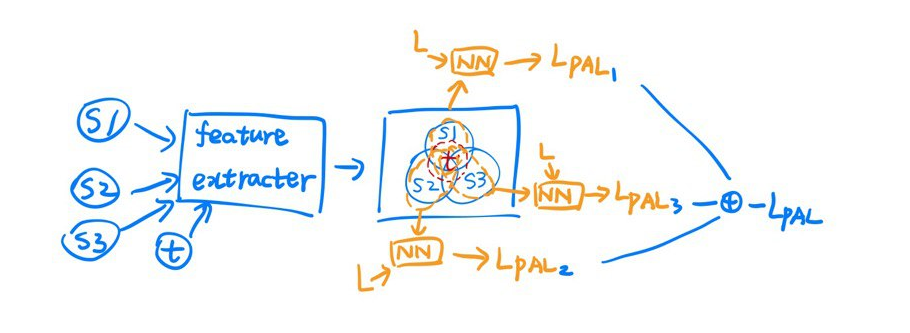
\includegraphics{Week03_PAL.png}
                    \caption{Partial Alignment Loss的计算}
                    \label{fig:PAL}
                \end{figure}
            \subsubsection{代码实现}
                构建一个两层FC的PAN(Partial Alignment Network)网络用于学习 $v$ ,
                使用M3SDA模型中原有的k\_moment进行Loss的计算。
                \begin{verbatim}
    # Partial Alignment Network
    class PAN(nn.Module):
        def __init__(self):
            # batch_size = 128, feature_n = 2048
            super(PAN, self).__init__()
            self.fc1 = nn.Linear(2048, 1024)
            self.fc2 = nn.Linear(1024, 2048)

        def forward(self, x):
            x = self.fc1(x)
            x = F.relu(x)
            x = self.fc2(x)
            x = F.relu(x)
            return x


    # Partial Alignment Loss
    def PAL(f_s, f_t, pan):
        v = pan(torch.abs(f_s - f_t))
        return mmd.linear_mmd2(f_s * v, f_t * v)


    # Partial Alignment Loss (All domain)
    def PAL_All(f_s1, f_s2, f_s3, f_s4, f_t, pan):
        # use k_moment
        v1 = pan(torch.abs(f_s1 - f_t))
        v2 = pan(torch.abs(f_s2 - f_t))
        v3 = pan(torch.abs(f_s3 - f_t))
        v4 = pan(torch.abs(f_s4 - f_t))
        v = (v1 + v2 + v3 + v4) / 4
        R = torch.sum((1 - v) ** 2)
        return msda.k_moment(f_s1 * v1, f_s2 * v2, f_s3 * v3, f_s4 * v4, \
                            f_t * v, k=4) + 1e-2 * R
                \end{verbatim}

        \subsection{负向网络Negative Purpose Network}
            之前设想过一个“帮倒忙的网络”,暂时叫做负向网络吧,后面仔细分析之后,
            觉得这个负向网络更像是一个子网的结构。
            \subsubsection{训练方法}
                以最简单的情况为例,假设在特征提取器的最后一层后面再加上一个“混淆层”,
                用于干扰提取的特征,而分类器为了获得正确的结果,则需要对特征有更深入的分析,
                当训练结束后,去掉“混淆层”,由于分类器的分析能力已经很强了,
                此时又获得了更为准确的特征,可能会得到更好的结果。

                至于“混淆层”的训练,可以认为其更新规则恰好跟主网络是相反的,
                即与主网络使用同一个Loss,而参数更新的时候朝着Loss增大的方向。
                负向网络的输出的数量级应该比主网络小,这样才不容易造成过大负面影响而导致训练失败。

                为了保证Negative Purpose Network(NPN)仅对主网络造成很微小的影响,
                引入如下regularization:

                $$
                    R(x) = \sum_{i=1}^n L(f(x)_i, x_i)
                $$

                其中 $f$ 表示NPN,$x$ 表示前面网络传来的 $n$ 维向量(feature vector)。

                暂时对这方面没有想到Loss相关的设计,感觉上可以把它当作一种训练技巧或者模型结构
                (后续根据实验的效果再考虑用不用)。
    \section{疑问/困难}
        \begin{enumerate}
            \item 对于负向网络的设计感觉不太完善,还有些简陋
            \item 尽管实现了PAL的代码,但是初期实验的结果并不理想(原模型训练3 epoch接近稳定,正确率达74\%,
            而修改后的模型训练10 epoch后仍未稳定,正确率仅65\%;可能是因为没有详细调参,也可能是设计或者实现上出了问题)
        \end{enumerate}
\end{document}
